\section{期望的积分表示}
\label{sec:pspace-expectation}

第~\ref{chap:random-variable-moments}章把期望定义为概率表上的加权和或密度的积分，等待时间$W$只能把两部分拆开计算，Cantor变量的期望则无从下手。另外几个结论也留了下来：两个任意随机变量之和的期望、求和与取极限的交换、用密度直接计算$\mathbb{E}[g(X)]$的公式。这些都归结为同一件事：期望是随机变量对概率测度的积分。

\paragraph{非负随机变量}
最简单的随机变量只取有限个值。设$A_1,\dots,A_m$是$\Omega$的一个划分，各块都是事件，$a_i\geq0$，
\[
  X=\sum_{i=1}^{m}a_i\mathbf{1}_{A_i}.
\]
这样的$X$称为简单随机变量，它在每一块上取常数值。它的期望只能是按块加权：
\[
  \mathbb{E}[X]=\sum_{i=1}^{m}a_i\,\mathbb{P}(A_i),
\]
这与第~\ref{chap:random-variable-moments}章对有限取值变量的定义一致。一般的非负随机变量用从下方逼近它的简单随机变量来定义，这就是卷四对非负可测函数的积分。

\begin{definition}[非负随机变量的期望]
\label{def:pspace-expectation-nonnegative}
设$X\geq0$是随机变量。称
\begin{equation}
  \mathbb{E}[X]=\int_{\Omega}X\,\mathrm{d}\mathbb{P}=\sup\bigl\{\mathbb{E}[\varphi]:\ \varphi\text{ 是简单随机变量},\ 0\leq\varphi\leq X\bigr\}
  \label{eq:pspace-expectation-nonnegative}
\end{equation}
为$X$的期望，它的值属于$[0,+\infty]$。
\end{definition}

上确界并不需要逐个比较。卷四给出了一列标准的逼近：
\begin{equation}
  \varphi_n=\min\Bigl\{n,\ \frac{\lfloor2^{n}X\rfloor}{2^{n}}\Bigr\},\qquad n=1,2,\dots .
  \label{eq:pspace-simple-approx}
\end{equation}
$\varphi_n$把$X$的取值向下取整到$2^{-n}$的整数倍，并在$n$处截断，它只取有限个值，且$\varphi_n\uparrow X$。由单调收敛定理，$\mathbb{E}[\varphi_n]\uparrow\mathbb{E}[X]$。

这个逼近与黎曼积分的思路不同。黎曼积分切分的是定义域，在$\Omega$上切小块；这里切分的是取值，把$X$的值分成宽$2^{-n}$的层，每层的值乘以落在这层的概率再相加。$\Omega$可以是任何集合，没有“小块”可言，按取值分层却总能进行，所需的只是每层$\{k2^{-n}\leq X<(k+1)2^{-n}\}$是事件，也就是$X$的可测性。

在木棍模型上看$X(\omega)=-\ln(1-\omega)$，它服从$\operatorname{Exp}(1)$。$n=1$时$\varphi_1$取三个值，
\[
  \varphi_1=\begin{cases}0,&X<\tfrac12,\\ \tfrac12,&\tfrac12\leq X<1,\\ 1,&X\geq1,\end{cases}
\]
各层的概率由指数分布的尾概率算出，于是
\[
  \mathbb{E}[\varphi_1]=\tfrac12\bigl(\mathrm{e}^{-1/2}-\mathrm{e}^{-1}\bigr)+1\cdot\mathrm{e}^{-1}\approx0.1193+0.3679=0.4872 .
\]
继续加细，前几项依次为
\[
  \mathbb{E}[\varphi_1]\approx0.4872,\quad \mathbb{E}[\varphi_2]\approx0.7611,\quad \mathbb{E}[\varphi_3]\approx0.8921,\quad \mathbb{E}[\varphi_4]\approx0.9513,
\]
它们递增地趋于$\mathbb{E}[X]=1$（图~\ref{fig:pspace-simple-approx}）。

\begin{BookInlineFigure}
  \centering
  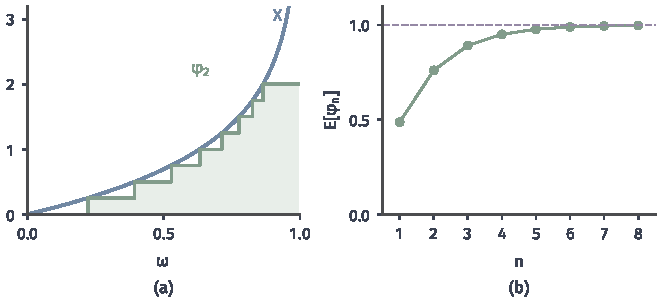
\includegraphics[width=112mm]{figures/07-probability/02-measure-theoretic-probability/matplotlib/pspace-simple-approx/figure.pdf}
  \caption{用简单随机变量逼近期望。(a)蓝线是$X(\omega)=-\ln(1-\omega)$，绿色阶梯是$\varphi_2$：取值向下取整到$1/4$的倍数并在$2$处截断，浅绿面积是$\mathbb{E}[\varphi_2]$；(b)绿点是$\mathbb{E}[\varphi_n]$，由式~\eqref{eq:pspace-simple-approx}按层精确算出，递增地趋于紫色虚线$\mathbb{E}[X]=1$。}
  \label{fig:pspace-simple-approx}
\end{BookInlineFigure}

\paragraph{有符号随机变量}
一般的随机变量拆成正部与负部，$X=X^{+}-X^{-}$，其中$X^{+}=\max\{X,0\}$，$X^{-}=\max\{-X,0\}$，两者都非负。

\begin{definition}[期望与可积]
\label{def:pspace-expectation}
设$X$是随机变量。若$\mathbb{E}[X^{+}]$与$\mathbb{E}[X^{-}]$至少有一个有限，定义
\begin{equation}
  \mathbb{E}[X]=\mathbb{E}[X^{+}]-\mathbb{E}[X^{-}].
  \label{eq:pspace-expectation}
\end{equation}
若$\mathbb{E}[X^{+}]$与$\mathbb{E}[X^{-}]$都有限，即$\mathbb{E}[\lvert X\rvert]<\infty$，称$X$可积。
\end{definition}

两部分都为无穷时期望没有定义，这正是第~\ref{chap:common-distributions}章对Cauchy分布的结论。可积的随机变量构成一个向量空间，期望是它上面的线性函数。

\begin{theorem}[期望的基本性质]
\label{thm:pspace-expectation-properties}
设$X,Y$是可积随机变量，$a,b\in\mathbb{R}$。
\begin{enumerate}
  \item 线性：$aX+bY$可积，且
  \begin{equation}
    \mathbb{E}[aX+bY]=a\,\mathbb{E}[X]+b\,\mathbb{E}[Y];
    \label{eq:pspace-linearity}
  \end{equation}
  \item 保序：若$X\leq Y$几乎必然成立，则$\mathbb{E}[X]\leq\mathbb{E}[Y]$；
  \item 绝对值估计：$\lvert\mathbb{E}[X]\rvert$不超过$\mathbb{E}[\lvert X\rvert]$；
  \item 若$X=Y$几乎必然成立，则$\mathbb{E}[X]=\mathbb{E}[Y]$；
  \item 若$X\geq0$且$\mathbb{E}[X]=0$，则$X=0$几乎必然成立。
\end{enumerate}
\end{theorem}

\begin{proof}
前四条是卷四积分的线性、单调性、绝对值估计以及“几乎处处相等的函数积分相同”，只是把测度取为$\mathbb{P}$。

第五条用一个分层估计。对正整数$n$，在$\{X>1/n\}$上$X>1/n$，在其余位置$X\geq0$，所以$\frac1n\mathbf{1}_{\{X>1/n\}}\leq X$。取期望，
\[
  \frac1n\,\mathbb{P}(X>1/n)\leq\mathbb{E}[X]=0 .
\]
于是每个$\{X>1/n\}$都是零概率事件。$\{X>0\}$是它们对$n$的并，由引理~\ref{lem:pspace-countable-null}，$\mathbb{P}(X>0)=0$。
\end{proof}

线性不要求知道$X$与$Y$的联合分布，也不要求它们独立：积分在每个样本点上逐点相加，$X(\omega)+Y(\omega)$在哪里取什么值，期望都按同一个$\mathbb{P}$加权。第~\ref{chap:random-variable-moments}章只对概率表证明了这一点，现在它对一切可积随机变量成立。

第五条补上第~\ref{chap:random-variable-moments}章关于方差的结论。设$X$平方可积且
\[
  \operatorname{Var}(X)=\mathbb{E}\bigl[(X-\mathbb{E}[X])^{2}\bigr]=0 .
\]
对非负变量$(X-\mathbb{E}[X])^{2}$用第五条，得$X=\mathbb{E}[X]$几乎必然成立。方差为零的随机变量几乎必然是常数，它在零概率事件上可以取别的值，但这不影响任何概率和期望。

\paragraph{期望与极限}
第~\ref{chap:random-variable-moments}章指出，对无穷多个随机变量之和逐项取期望，相当于交换求和与取极限的次序，需要额外的条件。卷四的两个收敛定理给出了这些条件，这里用概率的语言写出来。

\begin{theorem}[单调收敛与支配收敛]
\label{thm:pspace-convergence}
设$X_1,X_2,\dots$与$X$是随机变量，$X_n\to X$几乎必然成立。
\begin{enumerate}
  \item 若$0\leq X_1\leq X_2\leq\cdots$几乎必然成立，则
  \begin{equation}
    \lim_{n\to\infty}\mathbb{E}[X_n]=\mathbb{E}[X];
    \label{eq:pspace-monotone-convergence}
  \end{equation}
  \item 若存在可积的$Y$，使$\lvert X_n\rvert\leq Y$对每个$n$几乎必然成立，则$X$可积，且
  \begin{equation}
    \lim_{n\to\infty}\mathbb{E}[X_n]=\mathbb{E}[X].
    \label{eq:pspace-dominated-convergence}
  \end{equation}
\end{enumerate}
\end{theorem}

这是卷四单调收敛定理与支配收敛定理在概率测度下的特例。条件中的“几乎必然”无关紧要：由引理~\ref{lem:pspace-countable-null}，可数个几乎必然的条件同时在一个零概率事件之外成立，在那里把各变量改为$0$，期望都不变。

对非负随机变量列$Y_1,Y_2,\dots$，把单调收敛用于部分和$X_n=\sum_{k\leq n}Y_k$，得到
\begin{equation}
  \mathbb{E}\Bigl[\sum_{k=1}^{\infty}Y_k\Bigr]=\sum_{k=1}^{\infty}\mathbb{E}[Y_k],
  \label{eq:pspace-series-exchange}
\end{equation}
两边可以同为$+\infty$。若$Y_k$不一定非负，但$\sum_k\mathbb{E}[\lvert Y_k\rvert]<\infty$，则由式~\eqref{eq:pspace-series-exchange}，$Z=\sum_k\lvert Y_k\rvert$可积，它控制全部部分和，支配收敛给出同样的交换。一个常用的推论是：取值于$\{0,1,2,\dots\}$的随机变量$T$可以写成$T=\sum_{k\geq1}\mathbf{1}_{\{T\geq k\}}$，因为$T=m$时恰有$k=1,\dots,m$这$m$项为$1$。由式~\eqref{eq:pspace-series-exchange}，
\[
  \mathbb{E}[T]=\sum_{k=1}^{\infty}\mathbb{P}(T\geq k).
\]
对首次出现正面的次数$T$，$\mathbb{P}(T\geq k)$是前$k-1$次都是反面的概率$2^{-(k-1)}$，所以
\[
  \mathbb{E}[T]=\sum_{k=1}^{\infty}2^{-(k-1)}=2 .
\]

没有单调性或支配函数时，交换可能失败。在木棍模型上令$X_n=n\,\mathbf{1}_{(0,1/n)}$。对每个$\omega$，只要$n>1/\omega$就有$X_n(\omega)=0$，而$X_n(0)=0$，所以$X_n\to0$处处成立。可是
\[
  \mathbb{E}[X_n]=n\cdot\frac1n=1\quad\text{对每个}n,
\]
极限的期望是$0$，期望的极限是$1$。质量$1$被挤进越来越窄的区间，最后从每个固定位置“逃走”了；任何控制函数都要不小于$\sup_nX_n$，它在$(\frac1{k+1},\frac1k)$上至少为$k$，期望是发散的调和级数，不可积。

\paragraph{分布积分公式}
期望定义在$\Omega$上，计算却几乎总是在取值空间上进行。下面的公式说明这样做总是合法的，它是卷四推前积分恒等式在概率中的形式。

\begin{theorem}[分布积分公式]
\label{thm:pspace-law-integral}
设$X$是取值于$(E,\mathcal{E})$的随机对象，$g:E\to\mathbb{R}$可测。若$g\geq0$，或$g(X)$可积，则
\begin{equation}
  \mathbb{E}\bigl[g(X)\bigr]=\int_{E}g\,\mathrm{d}P_X .
  \label{eq:pspace-law-integral}
\end{equation}
\end{theorem}

\begin{proof}
沿着积分的定义逐步推广。若$g=\mathbf{1}_{B}$，$B\in\mathcal{E}$，则$g(X)=\mathbf{1}_{\{X\in B\}}$，两边都等于$\mathbb{P}(X\in B)=P_X(B)$。由线性，式~\eqref{eq:pspace-law-integral}对非负简单函数成立。

对非负可测的$g$，取非负简单函数$g_n\uparrow g$，则$g_n(X)$也是递增到$g(X)$的非负简单随机变量。两边分别用单调收敛定理，
\[
  \mathbb{E}\bigl[g(X)\bigr]=\lim_{n\to\infty}\mathbb{E}\bigl[g_n(X)\bigr]=\lim_{n\to\infty}\int_Eg_n\,\mathrm{d}P_X=\int_Eg\,\mathrm{d}P_X .
\]

对一般的$g$，把非负情形分别用于$g^{+}$和$g^{-}$。$g(X)$可积时两部分都有限，相减即得。
\end{proof}

公式的右边只含$P_X$，所以期望只依赖分布：同分布的随机变量期望相同，$X$定义在哪个概率空间上无关紧要。它还说明，计算$\mathbb{E}[g(X)]$不必先求$g(X)$的分布，直接在$X$的分布上积分$g$即可。第~\ref{chap:random-variable-moments}章的公式都是它的特例。

若$X$取可数个值，$P_X=\sum_xp_X(x)\delta_x$，其中$\delta_x$是$x$处的单点测度，对单点测度积分就是取值，于是
\[
  \mathbb{E}\bigl[g(X)\bigr]=\sum_xg(x)\,p_X(x).
\]
若$X$有密度$f_X$，$P_X$是以$f_X$为密度的加权测度，卷四测度的密度一章的加权积分规则给出
\[
  \mathbb{E}\bigl[g(X)\bigr]=\int_{\mathbb{R}}g(x)\,f_X(x)\,\mathrm{d}x .
\]
这对任何使右边有意义的Borel函数$g$都成立，包括示性函数和分段常数函数，不需要$g(X)$有密度。

等待时间的分布式~\eqref{eq:pspace-waiting-law}是单点测度与加权测度之和，积分也分成两项。取$g(x)=x$与$g(x)=x^{2}$，
\[
  \mathbb{E}[W]=0.3\cdot0+0.7\int_0^{\infty}t\,\mathrm{e}^{-t}\,\mathrm{d}t=0.7,\qquad \mathbb{E}[W^{2}]=0.7\int_0^{\infty}t^{2}\,\mathrm{e}^{-t}\,\mathrm{d}t=1.4 .
\]
于是
\[
  \operatorname{Var}(W)=1.4-0.7^{2}=0.91 .
\]
第~\ref{chap:random-variable-moments}章“跳跃部分求和、连续部分积分”的做法，现在是对两个测度之和积分的线性。

\paragraph{尾积分公式}
非负随机变量的期望还可以只用尾概率表示。第~\ref{chap:tail-probabilities}章在有密度时证明过这一点，那里交换积分次序的依据是Tonelli定理；现在对一般的非负随机变量写出完整的论证。

\begin{theorem}[尾积分公式]
\label{thm:pspace-tail-integral}
设$X\geq0$是随机变量，则
\begin{equation}
  \mathbb{E}[X]=\int_0^{\infty}\mathbb{P}(X>t)\,\mathrm{d}t,
  \label{eq:pspace-tail-integral}
\end{equation}
两边可以同为$+\infty$。
\end{theorem}

\begin{proof}
把每个样本点上的取值写成一段长度：
\[
  X(\omega)=\int_0^{\infty}\mathbf{1}_{\{t<X(\omega)\}}\,\mathrm{d}t .
\]
被积函数是集合$G=\{(\omega,t):0\leq t<X(\omega)\}$在$\Omega\times[0,\infty)$中的示性函数。$G$是乘积$\sigma$代数中的集合：若$t<X(\omega)$，可以取有理数$q$使$t<q<X(\omega)$，反之亦然，所以
\[
  G=\bigcup_{q\in\mathbb{Q},\,q>0}\bigl(\{X>q\}\times[0,q)\bigr),
\]
这是可数个可测矩形之并。

于是$\mathbf{1}_{G}$是$\mathbb{P}\otimes\lambda$下的非负可测函数，Tonelli定理允许交换积分次序：
\[
  \mathbb{E}[X]=\int_{\Omega}\int_0^{\infty}\mathbf{1}_{G}(\omega,t)\,\mathrm{d}t\,\mathbb{P}(\mathrm{d}\omega)=\int_0^{\infty}\int_{\Omega}\mathbf{1}_{G}(\omega,t)\,\mathbb{P}(\mathrm{d}\omega)\,\mathrm{d}t .
\]
内层积分是$\mathbb{P}(X>t)$，即得式~\eqref{eq:pspace-tail-integral}。
\end{proof}

这个证明是在计算同一块区域面积的两种切法。用分位数变换把$W$实现为$Q_W(U)$，区域$G$就是$Q_W$的图像下方（图~\ref{fig:pspace-tail-integral}(a)）。竖着切，每条竖线的长度是$Q_W(u)$，对$u$积分得$\mathbb{E}[W]$；横着切，高度$t$处的横线长度是$\mathbb{P}(W>t)$，对$t$积分得尾积分。对$W$，
\[
  \int_0^{\infty}\mathbb{P}(W>t)\,\mathrm{d}t=\int_0^{\infty}0.7\,\mathrm{e}^{-t}\,\mathrm{d}t=0.7,
\]
与分布积分公式的结果一致。在$t=0$处，$\mathbb{P}(W>0)=0.7$而不是$1$，因为$W=0$的那部分质量对任何$t\geq0$都不在$\{W>t\}$中，它对期望没有贡献。

\begin{BookInlineFigure}
  \centering
  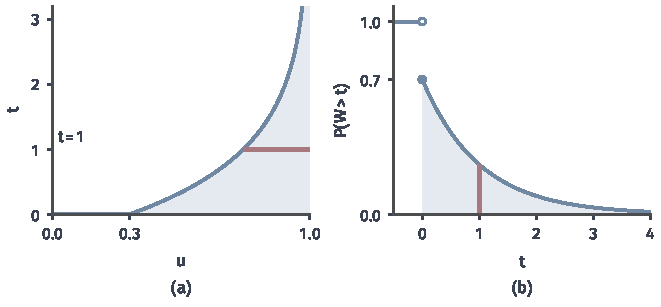
\includegraphics[width=112mm]{figures/07-probability/02-measure-theoretic-probability/matplotlib/pspace-tail-integral/figure.pdf}
  \caption{同一块面积的两种切法。(a)浅蓝区域在分位数函数$Q_W$的图像下方，红色横线是高度$t=1$处的切片，长度为$\mathbb{P}(W>1)=0.7\,\mathrm{e}^{-1}$；(b)蓝线是$\mathbb{P}(W>t)$，在$t=0$处从$1$降到$0.7$（实心点是函数值），红色竖线是同一个切片长度。两块浅蓝面积都等于$\mathbb{E}[W]=0.7$。}
  \label{fig:pspace-tail-integral}
\end{BookInlineFigure}

取值于非负整数时，$\mathbb{P}(T>t)$在每个区间$[k-1,k)$上等于$\mathbb{P}(T\geq k)$，式~\eqref{eq:pspace-tail-integral}就回到前面的级数公式$\mathbb{E}[T]=\sum_k\mathbb{P}(T\geq k)$。

\paragraph{独立对象的乘积期望}
第~\ref{chap:random-vectors}章对独立变量使用了$\mathbb{E}[XY]=\mathbb{E}[X]\,\mathbb{E}[Y]$，以及$\mathbb{E}[\phi(X,Y)]$的累次积分公式，在密度情形把它们当作计算规则。由乘积分布与分布积分公式，现在可以一般地证明。

\begin{theorem}[独立对象的期望]
\label{thm:pspace-independent-expectation}
设$X,Y$分别取值于$(E_1,\mathcal{E}_1)$与$(E_2,\mathcal{E}_2)$，相互独立，$\phi:E_1\times E_2\to\mathbb{R}$可测。若$\phi\geq0$，或$\phi(X,Y)$可积，则
\begin{equation}
  \mathbb{E}\bigl[\phi(X,Y)\bigr]=\int_{E_1}\Bigl(\int_{E_2}\phi(x,y)\,P_Y(\mathrm{d}y)\Bigr)P_X(\mathrm{d}x).
  \label{eq:pspace-independent-iterated}
\end{equation}
特别地，若实值随机变量$X,Y$独立且都可积，则$XY$可积，并且
\begin{equation}
  \mathbb{E}[XY]=\mathbb{E}[X]\,\mathbb{E}[Y].
  \label{eq:pspace-independent-product}
\end{equation}
\end{theorem}

\begin{proof}
由分布积分公式，$\mathbb{E}[\phi(X,Y)]$等于$\phi$对$P_{(X,Y)}$的积分。由定理~\ref{thm:pspace-independence-product}，$P_{(X,Y)}=P_X\otimes P_Y$。$\phi\geq0$时用Tonelli定理化为累次积分，即得式~\eqref{eq:pspace-independent-iterated}；$\phi(X,Y)$可积时用Fubini定理。

对乘积，先取$\phi(x,y)=\lvert x\rvert\lvert y\rvert\geq0$，内层积分是$\lvert x\rvert\,\mathbb{E}[\lvert Y\rvert]$，于是
\[
  \mathbb{E}\bigl[\lvert XY\rvert\bigr]=\mathbb{E}\bigl[\lvert X\rvert\bigr]\,\mathbb{E}\bigl[\lvert Y\rvert\bigr]<\infty,
\]
$XY$可积。再取$\phi(x,y)=xy$，用Fubini定理，内层积分是$x\,\mathbb{E}[Y]$，外层再积分得到式~\eqref{eq:pspace-independent-product}。
\end{proof}

用第~\ref{sec:pspace-independence}节的独立对$X\sim\operatorname{Unif}(0,1)$、$Y\sim\operatorname{Exp}(1)$算两个例子。由式~\eqref{eq:pspace-independent-product}，
\[
  \mathbb{E}[XY]=\tfrac12\cdot1=\tfrac12 .
\]
对$\phi(x,y)=\mathrm{e}^{-xy}$，它不是乘积形式，只能用累次积分。先对$y$积分，
\[
  \int_0^{\infty}\mathrm{e}^{-xy}\,\mathrm{e}^{-y}\,\mathrm{d}y=\frac{1}{1+x},
\]
再对$x$在$[0,1]$上积分，
\[
  \mathbb{E}\bigl[\mathrm{e}^{-XY}\bigr]=\int_0^1\frac{\mathrm{d}x}{1+x}=\ln2\approx0.6931 .
\]
式~\eqref{eq:pspace-independent-product}只是独立的一个推论，反过来不成立：第~\ref{chap:random-vectors}章已经看到，$\mathbb{E}[XY]=\mathbb{E}[X]\,\mathbb{E}[Y]$只说明不相关，不能推出独立。

\paragraph{Cantor变量的均值与方差}
最后回到章首的Cantor变量$X$，它等于$\sum_{k\geq1}2D_k/3^{k}$，其中$D_k$是第~\ref{sec:pspace-independence}节的独立公平比特。它既没有概率表也没有密度，可是$X$是非负随机变量，期望有定义。由式~\eqref{eq:pspace-series-exchange}，
\[
  \mathbb{E}[X]=\sum_{k=1}^{\infty}\frac{2\,\mathbb{E}[D_k]}{3^{k}}=\sum_{k=1}^{\infty}\frac{1}{3^{k}}=\frac12 .
\]
这与对称性一致：把每个$D_k$换成$1-D_k$，$X$变成$1-X$，而独立公平比特在这一替换下联合分布不变，所以$X\overset{\mathrm{d}}{=}1-X$。

方差要用支配收敛。令$\varepsilon_k=2D_k-1$，它等概率地取$\pm1$，各$\varepsilon_k$相互独立。记部分和
\[
  S_n=\sum_{k=1}^{n}\frac{\varepsilon_k}{3^{k}},\qquad \lvert S_n\rvert\leq\sum_{k=1}^{\infty}\frac{1}{3^{k}}=\frac12,
\]
它处处收敛到$X-\frac12$。展开平方，
\[
  \mathbb{E}[S_n^{2}]=\sum_{k=1}^{n}\frac{\mathbb{E}[\varepsilon_k^{2}]}{9^{k}}+\sum_{j\neq k}\frac{\mathbb{E}[\varepsilon_j\varepsilon_k]}{3^{j+k}}=\sum_{k=1}^{n}\frac{1}{9^{k}},
\]
其中$\varepsilon_k^{2}=1$，而$j\neq k$时$\varepsilon_j$与$\varepsilon_k$独立、均值为零，由式~\eqref{eq:pspace-independent-product}，交叉项的期望为零。

$S_n^{2}\to(X-\frac12)^{2}$处处成立，且$S_n^{2}\leq\frac14$，常数$\frac14$可积。由支配收敛定理，
\[
  \operatorname{Var}(X)=\lim_{n\to\infty}\mathbb{E}[S_n^{2}]=\sum_{k=1}^{\infty}\frac{1}{9^{k}}=\frac{1/9}{1-1/9}=\frac18 .
\]
标准差$\sqrt{1/8}\approx0.354$。图~\ref{fig:pspace-cantor-mean}是$20000$个模拟样本的直方图，样本均值约$0.498$，样本方差约$0.1250$。质量全部在Cantor集附近的若干小段上，均值$1/2$本身却落在中间被挖去的空隙里，没有任何样本能取到它；这再次说明期望是质量的重心，不必是可能的取值。

\begin{BookInlineFigure}
  \centering
  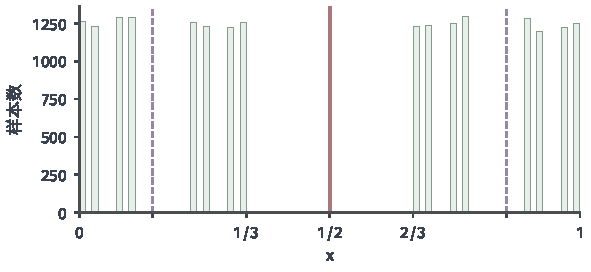
\includegraphics[width=100mm]{figures/07-probability/02-measure-theoretic-probability/matplotlib/pspace-cantor-mean/figure.pdf}
  \caption{Cantor变量的$20000$个模拟样本（每个样本保留$30$位三进制数字，种子$2026$），浅绿柱为$81$等分的直方图。红线是期望$1/2$，紫色虚线是$\frac12\pm\sqrt{1/8}$。样本都落在第二层保留的四段区间内，期望处于中间的空隙中。}
  \label{fig:pspace-cantor-mean}
\end{BookInlineFigure}

\paragraph{第一部分公式的来源}
表~\ref{tab:pspace-formula-sources}把第一部分的期望计算与它们在一般框架中的依据对应起来。每一行左边的公式，在第一部分只对概率表或密度验证过；右边的依据对任意分布都成立。

\begin{BookInlineTable}
  \centering
  \caption{第一部分的期望计算及其一般依据}
  \label{tab:pspace-formula-sources}
  \begin{tabular}{ll}
    \toprule
    第一部分的计算 & 一般框架中的依据 \\
    \midrule
    概率表求和$\sum_xg(x)p_X(x)$ & 分布积分公式，单点测度之和 \\
    密度积分$\int g(x)f_X(x)\,\mathrm{d}x$ & 分布积分公式，加权测度 \\
    混合分布分两部分计算 & 测度之和的积分 \\
    $\mathbb{E}[X+Y]=\mathbb{E}[X]+\mathbb{E}[Y]$ & 积分的线性 \\
    级数与期望交换 & 单调收敛、支配收敛 \\
    尾积分公式 & Tonelli定理 \\
    独立时$\mathbb{E}[XY]=\mathbb{E}[X]\,\mathbb{E}[Y]$ & 乘积分布与Fubini定理 \\
    \bottomrule
  \end{tabular}
\end{BookInlineTable}
